\section{Physical implications and falsifiable signatures of the fitted expansion history}
\label{sec:implications}

There is one present expansion rate only,
$H_{0,\mathrm{phys}} = \MXXVIIIHZeroPhys$\kmsMpc{} at background value
$\MXXVIIIHZeroBackground$\kmsMpc{} for the predecessor publication
fit (Sec.~\ref{sec:predecessor}; diagnostics of that frozen fit, not
of canonical Model~A). The epoch quantity is the expansion
rate $H(z)$ as a function of observed redshift; we never write an
epoch-dependent present rate and never describe the present rate as
changing between epochs. (Writing an epoch-indexed present rate would be
incorrect: the present rate is defined at $z_{\mathrm{obs}} = 0$ only.)
This section derives the kinematic implications of the frozen fitted
$H(z)$ and states how they can be falsified. Claim identities refer to
\path{paper/claims.yaml}: epoch structure (epoch-structure diagnostic) and the
deceleration diagnostic (deceleration diagnostic) are diagnostics only; the
phantom-like reading (phantom-like reading (conditional)) is conditional; growth
(growth prediction (not supported)) is not supported; drift (redshift-drift test (not established)) is
not established; matching (matching diagnostic) is supported; the exact
neighbourhood (exact-neighbourhood gate) needs review; calibrator invariance
(calibrator-invariance assumption) is an assumption of the declared contract.

\subsection{Localised epoch structure against two comparators}

The frozen fitted expansion history shows localised structure in
$H(z_{\mathrm{obs}})$ with $H > 0$ everywhere on the analysed interval:
expansion never reverses into contraction. A feature in a derivative
of a reconstructed function is not automatically an observable
signature: structure in $\dot{H}$, $q$, or $w_{\mathrm{eff}}$ is a
mathematical property of the interpolation until it is mapped into a
redshift-resolved observable (Sec.~\ref{sec:observable-signatures}).
Figure~\ref{fig:epoch-residual} (panel~A) shows the
frozen rate against two explicitly-named comparators at the same
observed redshift:
$(H_{\mathrm{model}} - H_{\mathrm{same\text{-}domain\,null}})/H_{\mathrm{same\text{-}domain\,null}}$,
where the comparator is the exact-valid $A_{E} = 0$ same-domain null,
and $(H_{\mathrm{model}} - H_{\mathrm{bg}})/H_{\mathrm{bg}}$, where
$H_{\mathrm{bg}} = H_{0,\mathrm{bg}}E_{\mathrm{bg}}$ is the model's own
smooth background (never called the same-domain null). The exact-valid
same-domain $A_{E} = 0$ comparator retains substantial localised
late-time kinematic structure of its own: sharp excursions are not
unique to the early-time extension
(\path{paper/evidence/m28_epoch_signatures/null_kinematic_sanity.json}).
No stable quantitative dynamical marker survives the required checks
($n_{\mathrm{stable}} = 0$, disposition
PARAMETERIZATION\_SENSITIVE): the localised
structure is a diagnostic of the frozen fit, not established epoch
behaviour. A residual-sign change (fitted rate above vs below a
comparator) is not the same object as a kinematic-transition marker: the
marker is $H^{2} + \dot{H} = 0$, i.e.\ the zero of the deceleration
diagnostic, not the zero of the residual. Figure~\ref{fig:epoch-q} (panel~B) shows the
deceleration diagnostic $q(z_{\mathrm{obs}})$ read directly from the
audit epoch curves, with all zero crossings provisional.

\subsection{Kinematic reading: super-acceleration interpretation only}

Where the diagnostic gives $\dot{H} > 0$, the kinematic effective
equation of state satisfies $w_{\mathrm{eff,kin}} < -1$ by the identity
$w_{\mathrm{eff}} = -1 - 2\dot{H}/(3H^{2})$. The width profiles show at
once that the extreme magnitudes are parameterization-sensitive: a
$9.2\times$ broadening of the razor width costs only
$\Delta\chi^{2} \approx +0.02$ while the spike amplitude collapses
$163 \to 18$, so no quantitative phantom amplitude is claimed. We
describe such intervals with a phantom-like, super-acceleration
interpretation of the fitted kinematics only. This is not a claim of a
fundamental phantom field, and it is not a claim of repeated phantom
crossings or of multiple back-to-back phantom eras. Any crossing is
accepted as a physical transition only after it survives the full check
set: exact-neighbor check, width above the resolution bound, boundary
clearance, convergence under refit perturbations, and survival against
independent observables. Until then every crossing is a provisional
diagnostic feature of one frozen fit, not an established era.

\subsection{Geometric implication, not a measured oscillation}

The scalar curvature of the effective background,
$R = 6(\dot{H} + 2H^{2})/c^{2}$, follows the fitted $H(z)$ and its
derivative as a geometric implication of the frozen background. It is
not a measured oscillation of spacetime: no independent curvature or
oscillation measurement is claimed here.

\subsection{BAO responses under the frozen-background constraint}

Figure~\ref{fig:epoch-bao} (panel~C) shows the fractional responses of the radial ($D_{H}$) and
transverse ($D_{M}$) BAO scales of the early-time $\Gamma(z)$ model relative to the
exact-valid same-domain ($A_{E} = 0$) null, sourced from the audit BAO
signature predictions. DESI is in-likelihood, so this comparison is an
overlay only (\texttt{validated\_external=false}), never independent validation. $D_{H}$ is local in the expansion rate while $D_{M}$ is
an integral over it, so the two respond differently to the same
localised $H(z)$ structure. The background is frozen: there
is no independent tuning of the BAO predictions beyond the frozen fit.

\begin{figure}[!htbp]
  \centering
  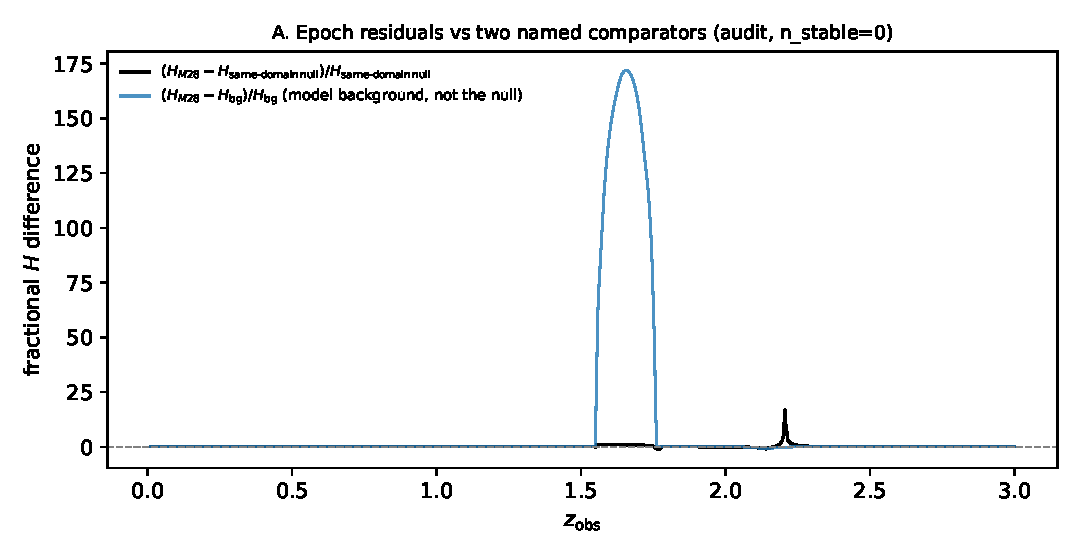
\includegraphics[width=0.85\linewidth]{figures/generated/figure_07A_epoch_residual.pdf}
  \caption{Epoch residual diagnostic for the frozen fitted
  $H(z_{\mathrm{obs}})$ against two explicitly-named comparators at the
  same observed redshift:
  $(H_{\mathrm{model}} - H_{\mathrm{same\text{-}domain\,null}})/H_{\mathrm{same\text{-}domain\,null}}$
  with the exact-valid $A_{E} = 0$ same-domain null, and
  $(H_{\mathrm{model}} - H_{\mathrm{bg}})/H_{\mathrm{bg}}$ with the model's
  own smooth background $H_{0,\mathrm{bg}}E_{\mathrm{bg}}$ (never called
  the null). The exact-valid null itself retains substantial localised
  late-time kinematic structure, so sharp excursions are not unique to
  the early-time extension. All early-time $\Gamma(z)$ markers provisional
  ($n_{\mathrm{stable}} = 0$).}
  \label{fig:epoch-residual}
\end{figure}

\begin{figure}[!htbp]
  \centering
  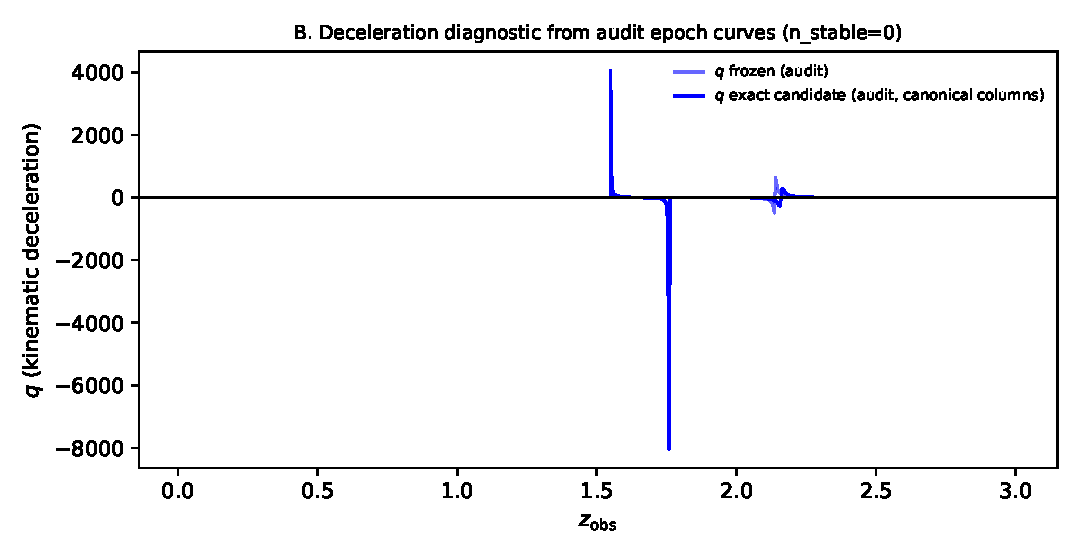
\includegraphics[width=0.85\linewidth]{figures/generated/figure_07B_epoch_q.pdf}
  \caption{Deceleration diagnostic $q(z_{\mathrm{obs}})$ read directly
  from the audit epoch curves (canonical columns; no finite-difference
  recomputation), frozen early-time $\Gamma(z)$ and exact candidate. Zero crossings
  provisional ($n_{\mathrm{stable}} = 0$); quantitative
  amplitudes and widths are parameterization-sensitive.}
  \label{fig:epoch-q}
\end{figure}

\begin{figure}[!htbp]
  \centering
  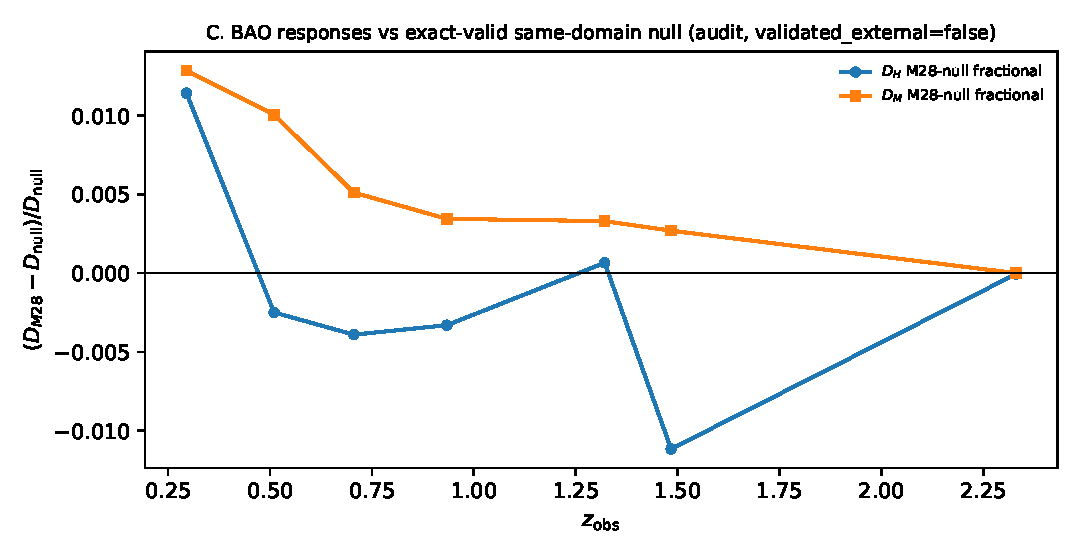
\includegraphics[width=0.85\linewidth]{figures/generated/figure_07C_epoch_bao.pdf}
  \caption{Fractional radial ($D_{H}$) and transverse ($D_{M}$) BAO
  responses of the early-time $\Gamma(z)$ model relative to the exact-valid same-domain
  ($A_{E} = 0$) null from the audit BAO signature predictions. DESI is
  in-likelihood: overlay only, \texttt{validated\_external=false}.
  Frozen background: no independent tuning.}
  \label{fig:epoch-bao}
\end{figure}
\FloatBarrier

\subsection{Predicted observable signatures}
\label{sec:observable-signatures}

Derivative features become testable only when mapped into
redshift-resolved observables. From the frozen fit with no refitting
(\path{paper/evidence/m28_epoch_observable_signatures/}):
radial BAO fractional response up to $\sim$$1.1$\% across 7 DESI bins
(overlay only, since DESI is in-likelihood there is no external
validation); transverse response up to
$\sim$$1.3$\%; distance-modulus signature
$|\Delta\mu| \lesssim 0.028$~mag from the $D_{M}$ ratio; and
background-projected redshift-drift curves
$\dot{z} = (1+z)H_{0} - H(z)$ for the model, the same-domain null,
and a $H_{0} = 67.4$\kmsMpc{} reference. The drift curves assume the
standard clock mapping and are provisional pending clock-mapping
validation -- they are the smoking-gun format, not yet a validated
number.

\subsection{Future falsification tests}

Because the background is frozen, each of the following is a genuine
prediction-then-comparison exercise (freeze, derive, compare beyond the
fit): cosmic-chronometer $H(z)$ points, independent BAO releases beyond
the fitted DESI block, standard-siren distances, redshift drift once the
clock mapping is validated (no numeric drift prediction is made here),
growth observables only after a perturbation sector exists, and lensing
observables only after the theory sector they require exists. Growth
has no perturbation sector here, so no growth numbers are quoted; the
qualitative statement is only that a future perturbation extension must
confront growth data.

\subsection{Falsification principle}

The rule is freeze, derive, compare beyond the fit: the 23-parameter
predecessor publication fit is frozen, its $H(z)$ implications are derived without
refitting, and they are compared against observables that did not enter
the fit. A failed comparison falsifies the localised structure.

\subsection{Limitations of this section}

The structures are derivative-fragile while the integrated distances
are robust: $q$, $\dot{H}$, and $w_{\mathrm{eff}}$ amplify spline
slope noise that the distance integrals average out. The matching at
$u = \ln 11$ is $C^{0}$ but not $C^{1}$ (C0-not-C1), so derivatives near
the kink are handled by masking, never by smoothing across. One
provisional width near $z \sim 1.54$ is razor-thin and sits near the
resolution bound. The exact neighbor of the frozen vector has not been
exhaustively mapped: a gate miss there, or an exact neighbor with equal
likelihood and different structure, would revise the markers. DESI is
not independent of the fit and cannot supply independent validation
of structures it helped fit. There is no growth sector, and drift is
pending clock-mapping validation (drift pending). The exact-valid null
sanity report
(\path{paper/evidence/m28_epoch_signatures/null_kinematic_sanity.json})
shows the same-domain null carries its own sharp late-time kinematic
structure ($\dot{H}$ zeros, $q$ zeros, narrow $q < 0$ widths), so
choppiness alone cannot establish model-specific epoch behaviour. In
short, the fitted history is a localized kinematic structure that is
falsifiable, but reality and character must survive the tests above.
